\documentclass[a4paper]{article}
\addtolength{\hoffset}{-2.25cm}
\addtolength{\textwidth}{4.5cm}
\addtolength{\voffset}{-3.25cm}
\addtolength{\textheight}{5cm}
\setlength{\parindent}{15pt}

\usepackage[unicode=true, colorlinks=false, hidelinks]{hyperref}
\usepackage[utf8]{inputenc}
\usepackage[english, russian]{babel}
\usepackage{mathtext}
\usepackage[T2A, TS1]{fontenc}
\usepackage{microtype} % Slightly tweak font spacing for aesthetics
\usepackage{amsthm, amssymb, amsmath, amsfonts, nccmath}
\usepackage{nicefrac}
\usepackage{epstopdf}
\usepackage[export]{adjustbox}
\usepackage{float} % Improved interface for floating objects
\usepackage{graphicx, multicol} % Enhanced support for graphics
\usepackage{pdfrender,xcolor}
\usepackage{breqn}
\usepackage{mathtools}
\usepackage{titling}
\usepackage{bm}
\usepackage{centernot}
\usepackage[cal=boondoxo,calscaled=.96]{mathalpha}
\usepackage{marvosym, wasysym} % More symbols
\usepackage{rotating} % Rotation tools
\usepackage{censor} % Facilities for controlling restricted text
\usepackage{indentfirst}
\usepackage{svg}

\DeclareMathOperator{\rad}{rad}
\DeclareMathOperator{\imid}{mid}
\DeclareMathOperator{\sign}{sign}
\newcommand{\mbb}[1]{\mathbb{#1}}
\newcommand{\mbf}[1]{\mathbf{#1}}

\usepackage{array}
\newcolumntype{C}[1]{>{\centering\let\newline\\\arraybackslash\hspace{0pt}}m{#1}}

\usepackage{fancyhdr}
\pagestyle{fancy}
\fancyhead{}\renewcommand{\headrulewidth}{0pt}
\fancyfoot[L]{}
\fancyhead{}
\fancyfoot{}
\fancyfoot[R]{\thepage}
\begin{document}
\large
\begin{center}
    Санкт-Петербургский политехнический университет\\
    Высшая школа прикладной математики и\\вычислительной физики,\\ 
    Физико-механический институт\\
    \vspace{3em}
    Направление подготовки\\
    01.03.02 «Прикладная математика и информатика»\\
    \vspace{10em}
    \Large
    Отчет по лабораторной работе №1 \\
    по дисциплине «Интервальный анализ»
    \vspace{19em}
    \large
\end{center}
Выполнил студент гр. 5030102/80201\\
Кирпиченко С. Р.\\
Руководитель\\
Баженов А. Н.
\vspace{10em}
\begin{center}
    Санкт-Петербург\\
    2021
\end{center}
\thispagestyle{empty}
\newpage
\tableofcontents
\addtocontents{toc}{~\hfill\textbf{Страница}\par}
\newpage
\listoffigures
\addtocontents{lof}{~\hfill\textbf{Страница}\par}
\newpage
\section{Постановка задачи}
\subsection{Линейная и полиномиальная регрессия}
Дана задача вида $\mathbf{y}=\mathbf{X}\beta$, в общей регрессионной постановке необходимо найти вектор $\beta$ и восстановить зависимости между рассматриваемыми величинами. В данной работе рассматривается вопрос установления особенности матрицы $\mathbf{X}$, так как в этом случае рассматриваемая ИСЛАУ становится неразрешимой. 

Дано 
\begin{equation}
    \mathrm{mid}\:\mathbf{X}=\begin{pmatrix}
      1& 1\\
      1.1& 1
    \end{pmatrix}
\end{equation}
Необходимо рассмотреть матрицу вида 
\begin{equation}\label{mat:reg}
\mathbf{X}=\begin{pmatrix}
  [1-\varepsilon,1+\varepsilon]& 1\\
  [1.1-\varepsilon,1.1+\varepsilon]& 1
\end{pmatrix}
\end{equation}
и определить, при каком значении $\varepsilon$ она содержит особенные точечные матрицы.
\subsection{Решение задач томографии}
При решении задач томографии появляются системы типа $\mathbf{A}x=\mathbf{b}$. В данной работе необходимо рассмотреть матрицу 
\begin{equation}\label{math:tom}
\mathbf{A}=\begin{pmatrix}
  [1-\varepsilon,1+\varepsilon]& [1-\varepsilon,1+\varepsilon]\\
  [1.1-\varepsilon,1.1+\varepsilon]& [1-\varepsilon,1+\varepsilon]
\end{pmatrix}
\end{equation}
и определить, при каком радиусе она содержит особенную матрицу. 
\subsection{Глобальная оптимизация}
Для функции МакКормика
\begin{equation}\label{macCorm}
    f(x,y)=\sin(x+y)+(x-y)^2-1.5x+2.5y+1,
\end{equation}
имеющей один глобальный экстреммум, и функции Химмельблау
\begin{equation}\label{Himmel}
    f(x, y) = (x^2 + y - 11)^2 + (x + y^2 - 7)^2,
\end{equation}
имеющей 4 равнозначных глобальных экстремума, необходимо провести вычисления по поиску глобального минимума с помощью простейшего интервального адаптивного алгоритма глобальной оптимизации.
\section{Теория}
\subsection{Выяснение радиуса элементов матрицы, при котором она становится особенной}
Интервальная матрица $\mathbf{A}$ - особенная, если $\exists A\in\mathbf{A}:\;\det(A)=0$, иначе - неособенная. 

$\mathrm{rad}\:\mathbf{A}=\{A\mid\:a_{ij}=\mathrm{rad}\:\mathbf{a}_{ij}\}$ - радиус интервальной матрицы $\mathbf{A}$, $\mathrm{mid}\:\mathbf{A}=\{A\mid\:a_{ij}=\mathrm{mid}\:\mathbf{a}_{ij}\}$ - середина интервальной матрицы $\mathbf{A}$.

$\mathrm{vert}\:\mathbf{A}=\{A\in\mathbf{A}\mid A=\{a_{ij}\}\;a_{ij}\in\{\underline{\mathbf{a}_{ij}},\overline{\mathbf{a}_{ij}}\}\}$ - множество вершин интервальной матрицы $\mathbf{A}$. 

$\sigma(A)$ - множество сингулярных чисел матрицы, вычисляемых как алгебраический квадратный корень из собственных значений матрицы $AA^T$.
\subsubsection{Критерий Баумана}
Матрица $\mathbf{A}\in\mathbb{IR}^{n\times n}$ неособенна $\Leftrightarrow\;\forall A',A''\in\mathrm{vert}\:\mathbf{A}\;\det(A')\cdot\det(A'')>0$ 
\subsubsection{Признак Румпа}
$\mathbf{A}\in\mathbb{IR}^{n\times n}$, $\sigma_{\mathrm{max}}(\mathrm{rad}\:\mathbf{A})<\sigma_{\mathrm{min}}(\mathrm{mid}\:\mathbf{A})\Rightarrow\mathbf{A}$ неособенна.
\subsection{Глобальная оптимизация}
Суть простейшего интервального адаптивного алгоритма глобальной оптимизации похожа на алгоритм дихотомии, только для многомерного случая. Имеется рабочий список рассматриваемых брусьев, для каждого из которых вычислено целевое значение функции (в интервальном смысле). На каждой итерации метод выбирает из этого списка брус, на котором нижняя оценка значения функции наименьшая. Этот брус удаляется из списка, после чего туда добавляются два новых, которые получились из исходного путем дробления его самой длинной компоненты пополам (от нижней границы до середины и от середины до верхней границы). На этих брусьях вычисляется интервальная оценка целевой функции, выполняется переход на новую итерацию.
\section{Реализация}
Для осуществления вычислений и визуализации результатов использовалась среда Matlab с библиотекой интервальной арифметики IntLab.
\section{Результаты}
\subsection{Линейная и полиномиальная регрессия}
Для того, чтобы точечная матрица была особенной, достаточно линейной зависимости ее строк. В случае рассматриваемой матрицы (\ref{mat:reg}) это означает, что нам достаточно добиться непустого пересечения интервалов $\mathbf{x}_{1 1}$ и $\mathbf{x}_{2 1}$. Очевидно, что это достижимо при $\varepsilon\geq0.05$. Проверим, что при $\varepsilon=0.05$ найдется особенная точечная матрица:
\begin{equation*}
    \mathbf{X}=\begin{pmatrix}
  [0.95,1.05]& 1\\
  [1.05,1.15]& 1
\end{pmatrix},\: X=\begin{pmatrix}
  1.05& 1\\
  1.05& 1
\end{pmatrix}\in\mathbf{X},\:\det(X)=0
\end{equation*}
Воспользуемся признаком Румпа.
\begin{equation*}
    \mathrm{rad}\:\mathbf{X}=\begin{pmatrix}
    \varepsilon&0\\
    \varepsilon&0
    \end{pmatrix}
\end{equation*}
\begin{equation*}
    \sigma(\mathrm{rad}\:\mathbf{X})=\{0,\varepsilon\sqrt{2}\},\:\varepsilon>0\Rightarrow\sigma_{\mathrm{max}}(\mathrm{rad}\:\mathbf{A})=\varepsilon\sqrt{2}
\end{equation*}
\begin{equation*}
    \sigma(\mathrm{mid}\:\mathbf{X})=\left\{\sqrt{\frac{421+21\sqrt{401}}{200}},\sqrt{\frac{421-21\sqrt{401}}{200}}\right\}\approx\{2.0512, 0.0488\}\Rightarrow\sigma_{\mathrm{min}}(\mathrm{mid}\:\mathbf{X})=0.0488
\end{equation*}
Можно сделать вывод, что при $\varepsilon\sqrt{2}<0.0488\Rightarrow\varepsilon<0.0345$ матрица $\mathbf{X}$ не будет особенной.

Также воспользуемся критерием Баумана. Множество $\mathrm{vert}\:\mathbf{X}$ содержит 4 точечные матрицы. Обозначим их определители за $\Delta_i,\:i=\overline{1,4}$ и сосчитаем.
\begin{equation*}
    \Delta_1=-0.1\quad\Delta_2=2\varepsilon-0.1\quad\Delta_3=-2\varepsilon-0.1\quad\Delta_4=-0.1
\end{equation*}
Из этих значений уникальными являются $\Delta_i,\:i=\{1,2,3\}$. С помощью критерия Баумана можно найти значения $\varepsilon$, для которых рассматриваемая матрица будет неособенной, а так как критерий является необходимым и достаточным условием, то дополнение найденного множества будет описывать все особенные матрицы $\mathbf{A}$.

$\Delta_1<0\:\forall\varepsilon$. Следовательно, для выполнения критерия необходимо потребовать, чтобы все остальные определители тоже были меньше 0. Учитывая $\varepsilon>0$, получаем множество $\varepsilon<0.05$. Таким образом, матрица $\mathbf{X}$ особенна $\forall\varepsilon\geq0.05$, что согласуется с предыдущими расчетами.
\subsection{Задача томографии}
Воспользуемся признаком Румпа. 
\begin{equation*}
    \mathrm{rad}\:\mathbf{A}=\begin{pmatrix}
    \varepsilon&\varepsilon\\
    \varepsilon&\varepsilon
    \end{pmatrix}\quad
    \mathrm{mid}\:\mathbf{A}=\begin{pmatrix}
    1&1\\
    1.1&1
    \end{pmatrix}\quad
\end{equation*}
\begin{equation*}
    \sigma(\mathrm{rad}\:\mathbf{A})=\{0,2\varepsilon\},\:\varepsilon>0\Rightarrow\sigma_{\mathrm{max}}(\mathrm{rad}\:\mathbf{A})=2\varepsilon
\end{equation*}
\begin{equation*}
    \sigma(\mathrm{mid}\:\mathbf{A})=\left\{\sqrt{\frac{421+21\sqrt{401}}{200}},\sqrt{\frac{421-21\sqrt{401}}{200}}\right\}\approx\{2.0512, 0.0488\}\Rightarrow\sigma_{\mathrm{min}}(\mathrm{mid}\:\mathbf{A})=0.0488
\end{equation*}
Можно сделать вывод, что при $2\varepsilon<0.0488\Rightarrow\varepsilon<0.0244$ матрица $\mathbf{A}$ не будет особенной.

Для решения задачи воспользуемся критерием Баумана. Множество $\mathrm{vert}\:\mathbf{A}$ содержит 16 точечных матриц. Обозначим их определители за $\Delta_i,\:i=\overline{1,16}$ и сосчитаем.
\begin{equation*}
    \Delta_1=0.1\varepsilon-0.1\quad\Delta_2=-2\varepsilon^2+2.1\varepsilon-0.1\quad\Delta_3=2\varepsilon^2-2.1\varepsilon-0.1\quad\Delta_4=2\varepsilon^2-1.9\varepsilon-0.1
\end{equation*}
\begin{equation*}
    \Delta_5=-2\varepsilon^2+2.1\varepsilon-0.1\quad\Delta_6=-0.1\varepsilon-0.1\quad\Delta_7=0.1\varepsilon-0.1\quad\Delta_8=4.1\varepsilon-0.1
\end{equation*}
\begin{equation*}
    \Delta_9=-4.1\varepsilon-0.1\quad\Delta_{10}=0.1\varepsilon-0.1\quad\Delta_{11}=-0.1\varepsilon-0.1\quad\Delta_{12}=-2\varepsilon^2-2.1\varepsilon-0.1
\end{equation*}
\begin{equation*}
    \Delta_{13}=2\varepsilon^2+2.1\varepsilon-0.1\quad\Delta_{14}=2\varepsilon^2+1.9\varepsilon-0.1\quad\Delta_{15}=-2\varepsilon^2-2.1\varepsilon-0.1\quad\Delta_{16}=-0.1\varepsilon-0.1
\end{equation*}
Из этих значений уникальными являются $\Delta_i,\:i=\{1,2,3,4,6,8,9,12,13,14\}$. С помощью критерия Баумана можно найти значения $\varepsilon$, для которых рассматриваемая матрица будет неособенной, а так как критерий является необходимым и достаточным условием, то дополнение найденного множества будет описывать все особенные матрицы $\mathbf{A}$.

Учитывая, что $\varepsilon>0$, получаем $\Delta_6<0\:\forall\varepsilon$. Следовательно, для выполнения критерия необходимо потребовать, чтобы все остальные определители тоже были меньше 0. Получаем следующее множество решений:
\begin{equation*}
    (0,1)\cap(0,0.0456)\cap(0,1.095)\cap(0,1)\cap(0,\infty)\cap(0,0.0244)\cap(0,\infty)\cap(0,\infty)\cap(0,0.0456)\cap(0,0.05)
\end{equation*}
То есть матрица $\mathbf{A}$ неособенна тогда и только тогда, когда $\varepsilon<\frac{1}{41}$. То есть $\forall\varepsilon\geq\frac{1}{41}$ матрица $\mathbf{A}$ будет содержать особенные точечные матрицы. Рассмотрим $\varepsilon=\frac{1}{41}$:
\begin{equation*}
\mathbf{A}=\begin{pmatrix}
  \left[\frac{40}{41},\frac{42}{41}\right]& \left[\frac{40}{41},\frac{42}{41}\right]\\[0.3em]
  \left[1\frac{31}{410},1\frac{51}{410}\right]& \left[\frac{40}{41},\frac{42}{41}\right]
\end{pmatrix}
\end{equation*}
\begin{equation*}
    A=\begin{pmatrix}
    1\frac{1}{41}&\frac{40}{41}\\[0.3em]
    1\frac{31}{410}&1\frac{1}{41}
    \end{pmatrix}\in\mathbf{A},\quad\det(A)=0
\end{equation*}
\subsection{Глобальная оптимизация}
\subsubsection{Функция с одним экстремумом}
Для функции (\ref{macCorm}) в качестве начального приближения был выбран брус $\begin{pmatrix}
[-1.5,\: 4]\\
[-3,\: 4]
\end{pmatrix}$. Для наглядности иллюстраций в этом и следующем численном эксперименте число итераций ограничено 200.
\begin{figure}[H]
    \centering
    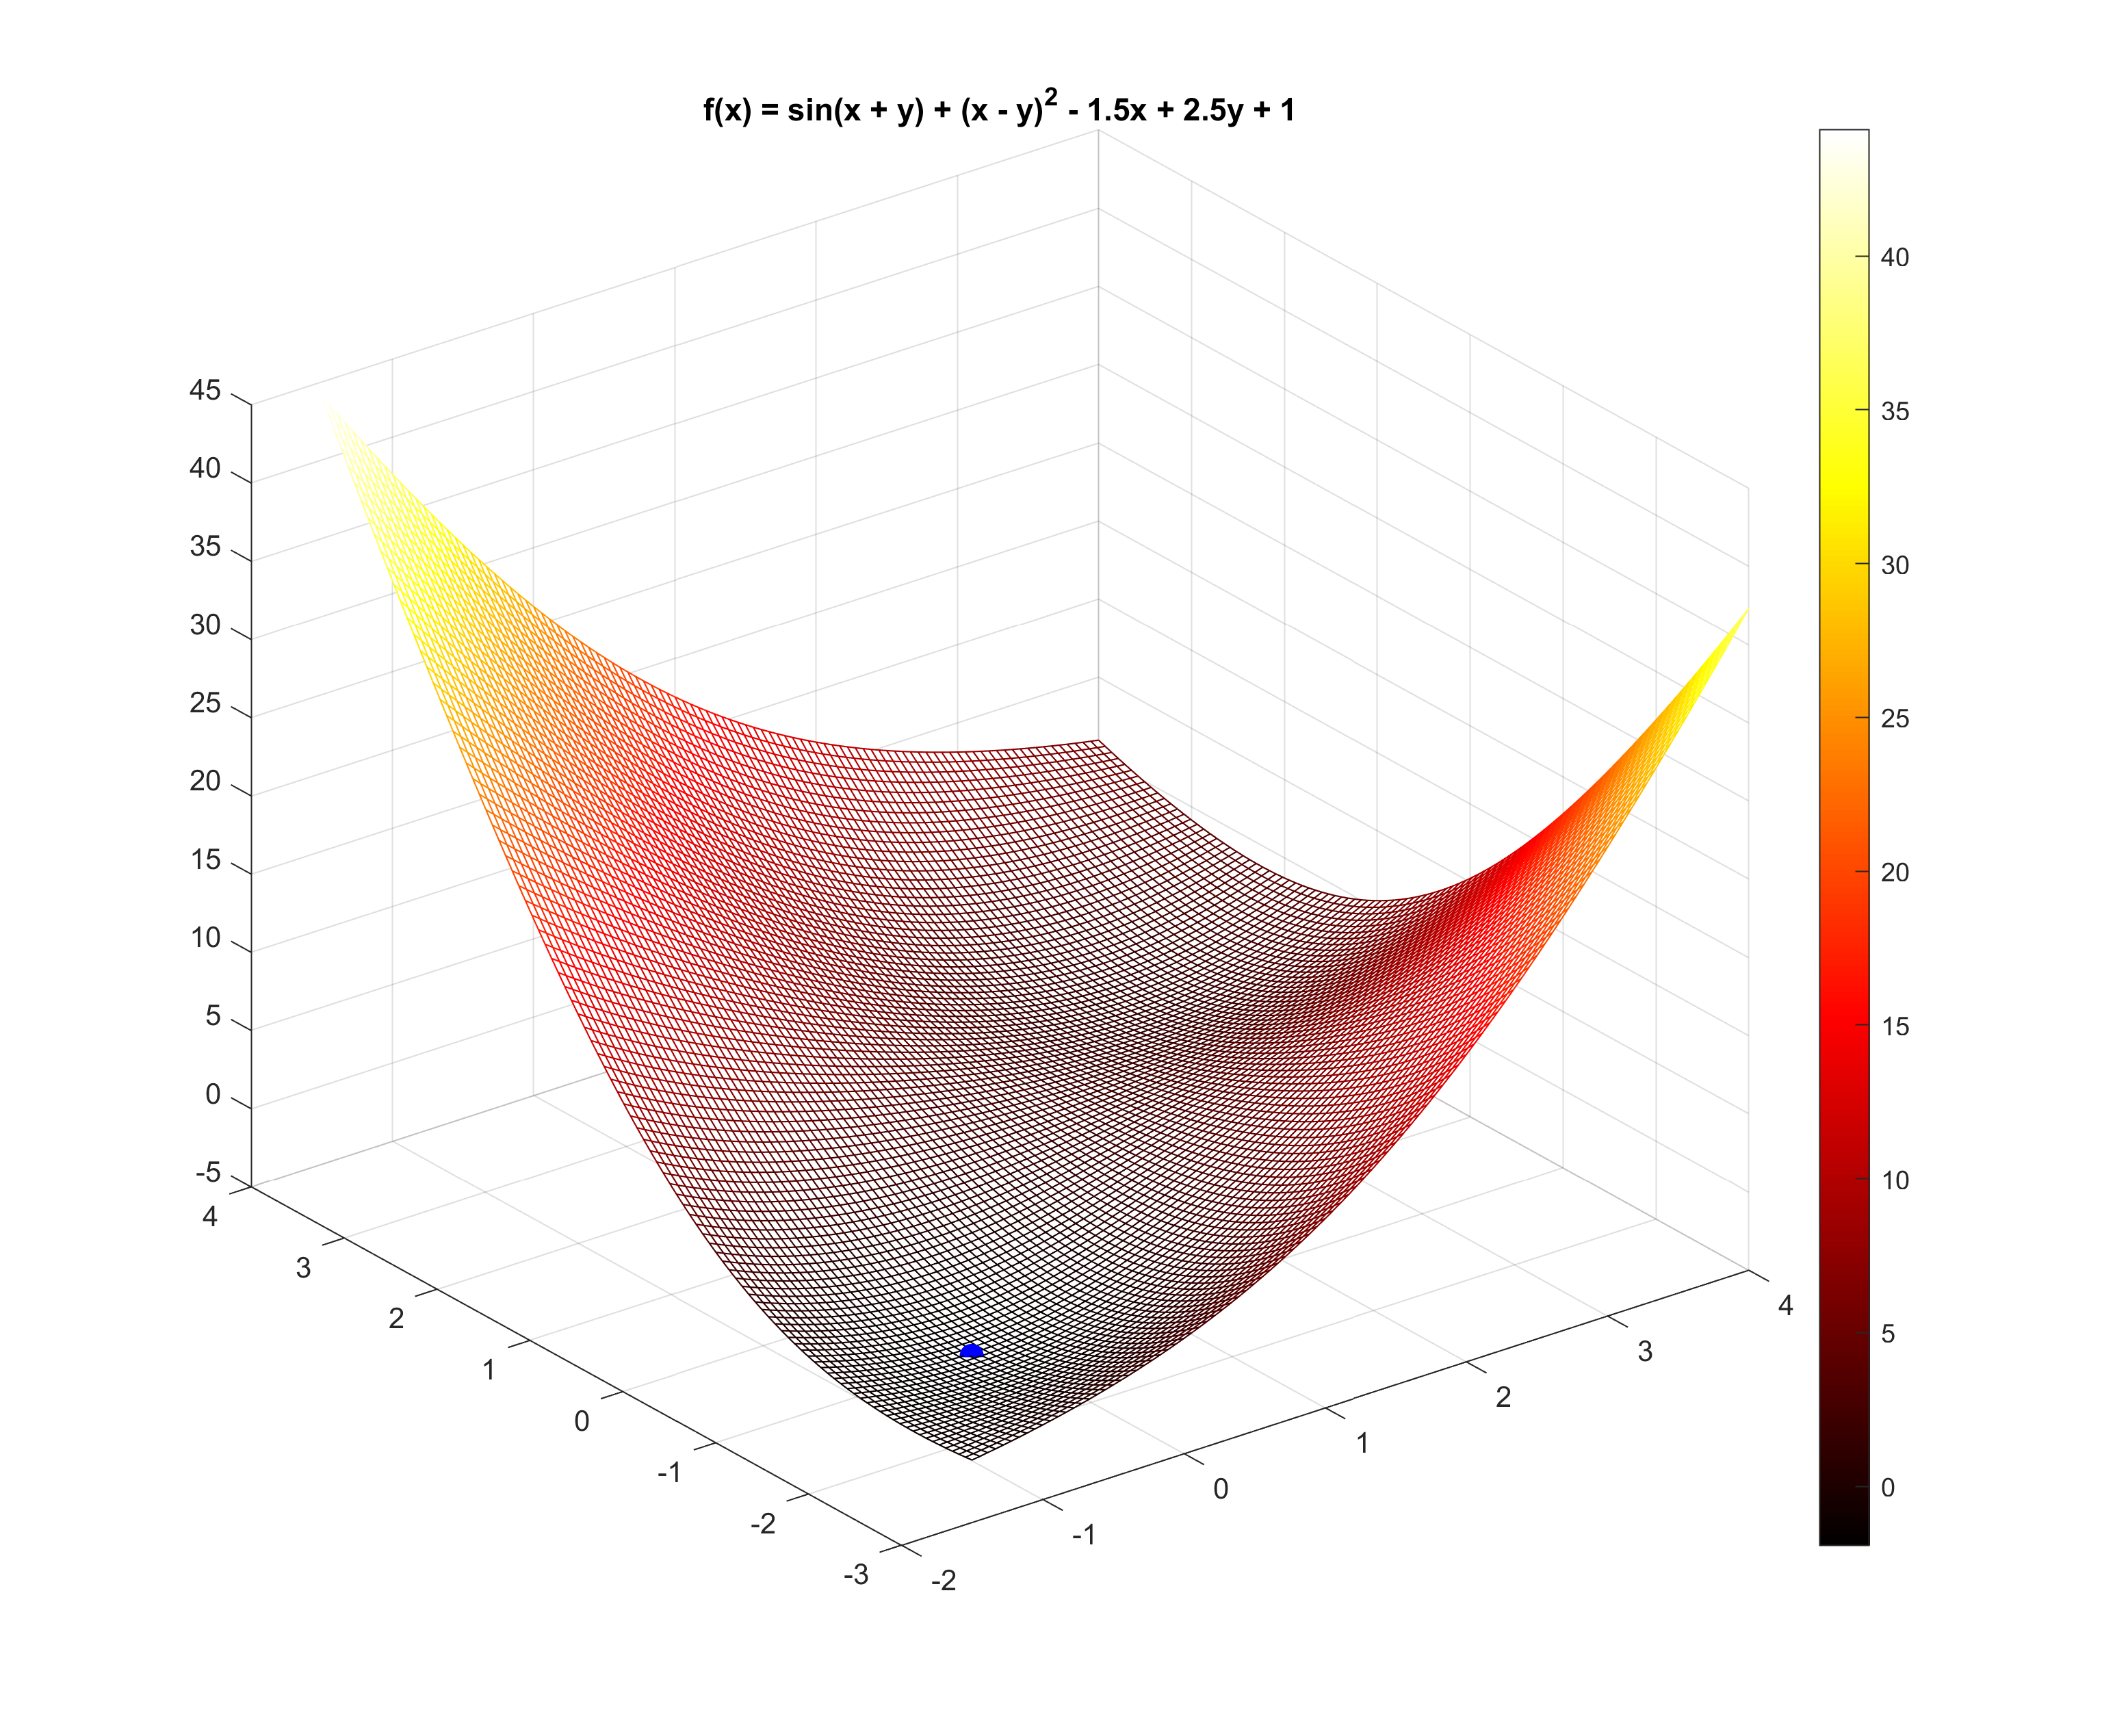
\includegraphics[width=13cm]{img/MacCormick3d.png}
    \caption{График функции МакКормика (\ref{macCorm})}
    \label{fig:macCorm}
\end{figure}
Минимум изображен на графике синей точкой. Получены следующие результаты:
\begin{figure}[H]
    \centering
    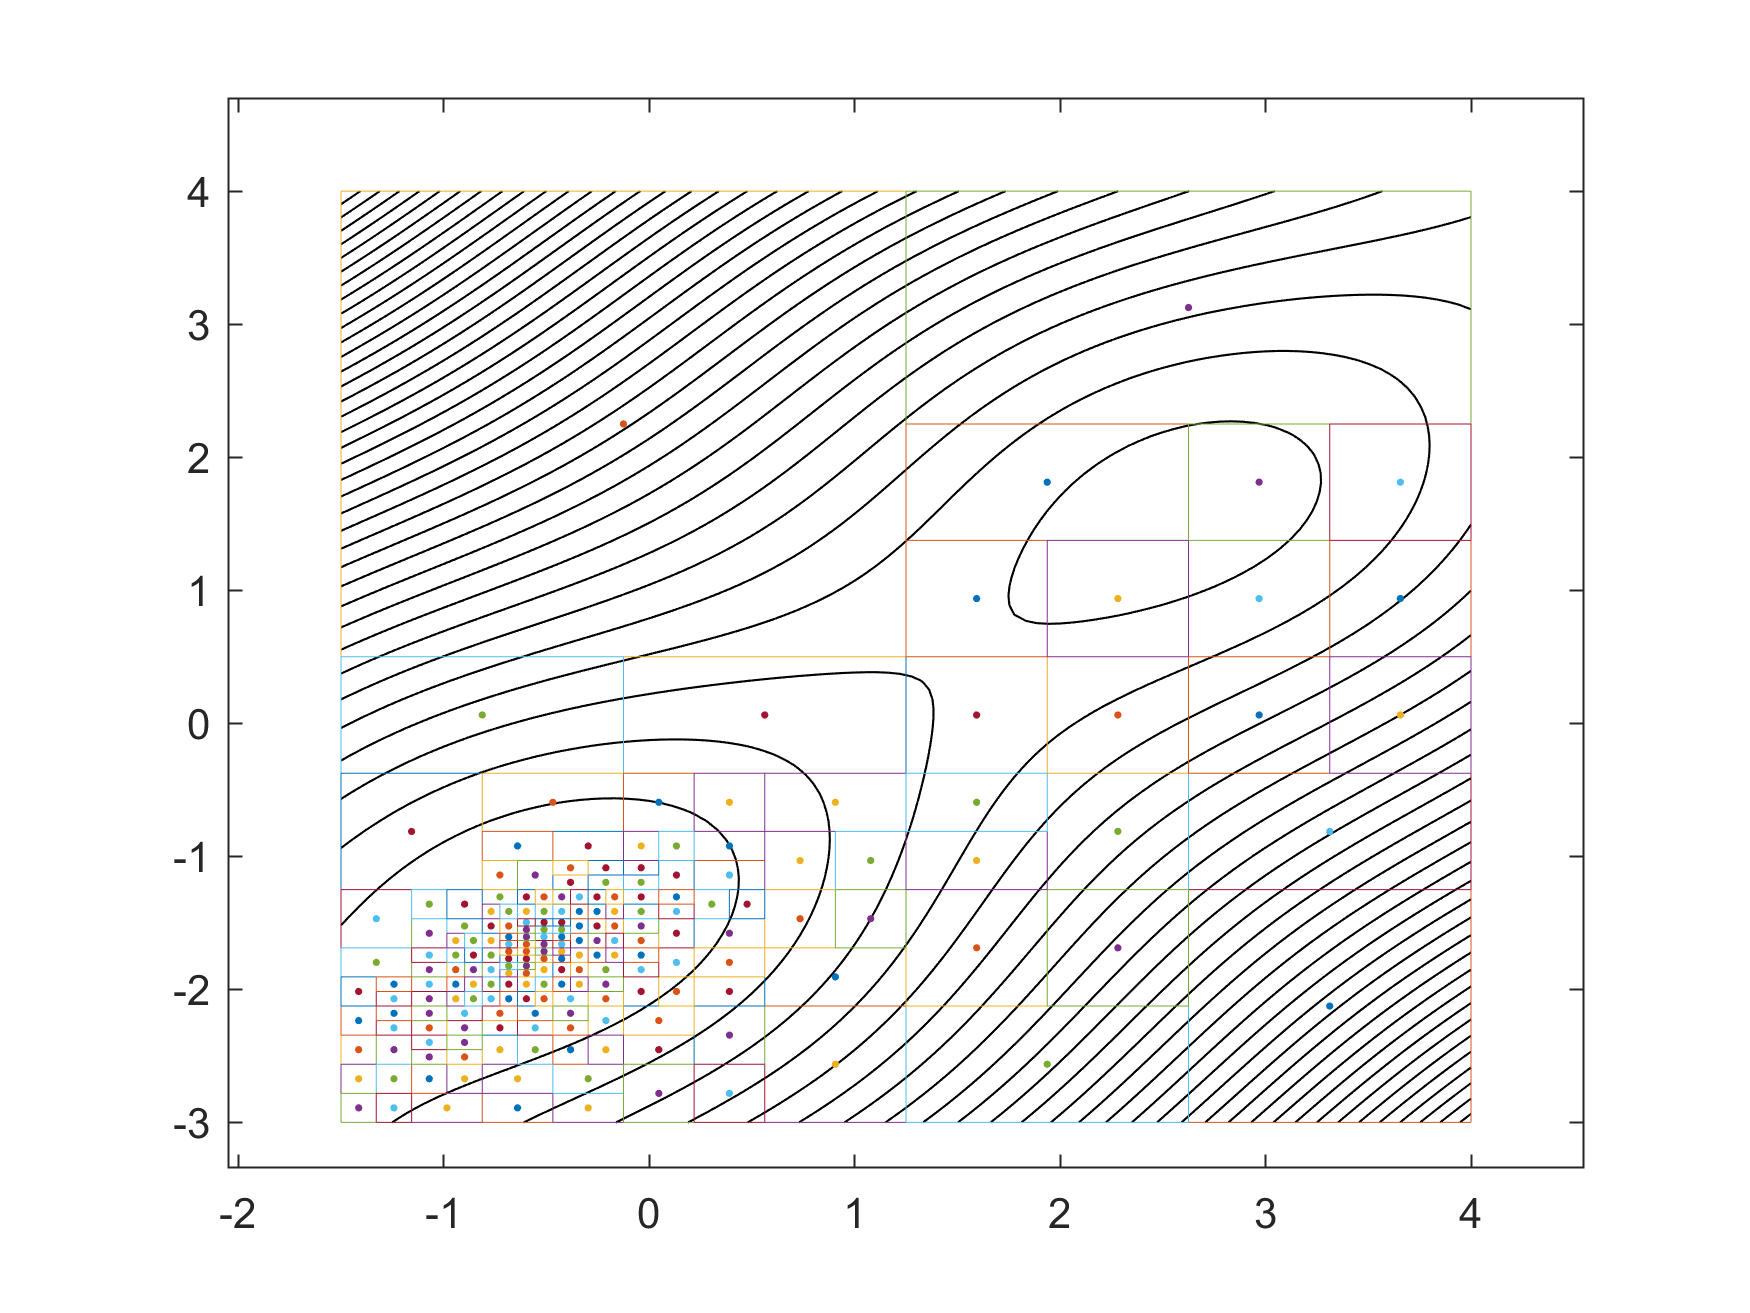
\includegraphics[width=13cm]{img/MacCormickOptim.png}
    \caption{Иллюстрация работы алгоритма для функции МакКормика (\ref{macCorm})}
    \label{fig:proc1}
\end{figure}
Как видим, число брусьев сгущается по мере приближения к экстремуму. В качестве ответа программа предлагает наименьшую нижнюю оценку значения функции за 200 итераций, поэтому в качестве итоговой оценки положения экстремума будет выбран брус, отвечающий этому значению $\mathbf{x}=\begin{pmatrix}
[   -0.3829,\:    -0.2968]\\ 
[   -1.5782,\:   -1.4687]
\end{pmatrix}$. Для него получаем значение функции $f(\mathbf{x})=[   -2.3019,    -1.3809]$. Точное значение минимума - $f(-0.5471, -1.5471)=-1.9133$. 

Проиллюстрируем работу алгоритма еще двумя графиками. Для их построения были взяты брусы из рабочего списка алгоритма. Для построения графика радиусов брусов бралась наибольшая компонента радиуса, так как в предложенном методе последующее дробление бруса производится по измерению, отвечающему наибольшей компоненте радиуса.
\begin{figure}[H]
    \centering
    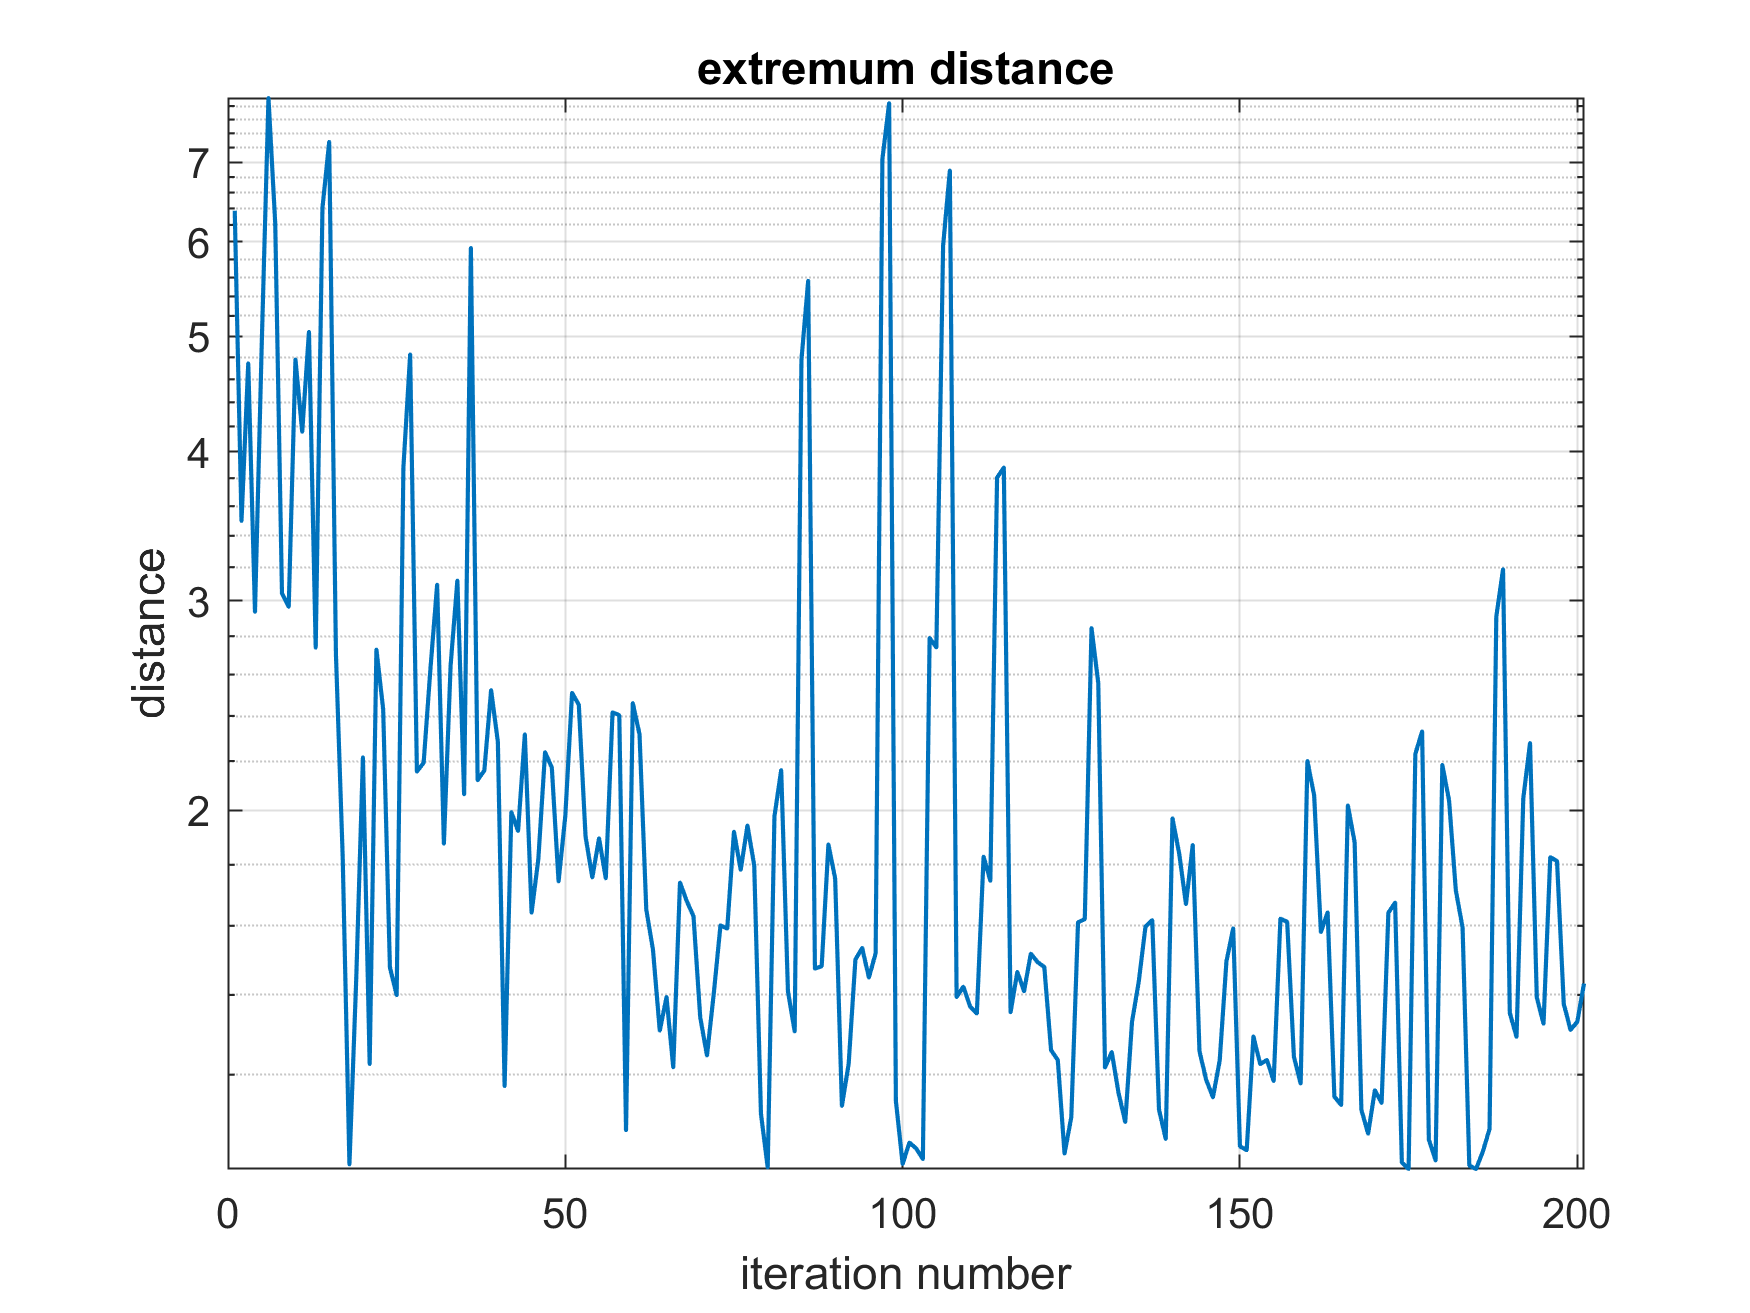
\includegraphics[width=15cm]{img/extr_dist.png}
    \caption{Расстояние до точки экстремума для функции МакКормика (\ref{macCorm})}
    \label{fig:mcExtr}
\end{figure}
\begin{figure}[H]
    \centering
    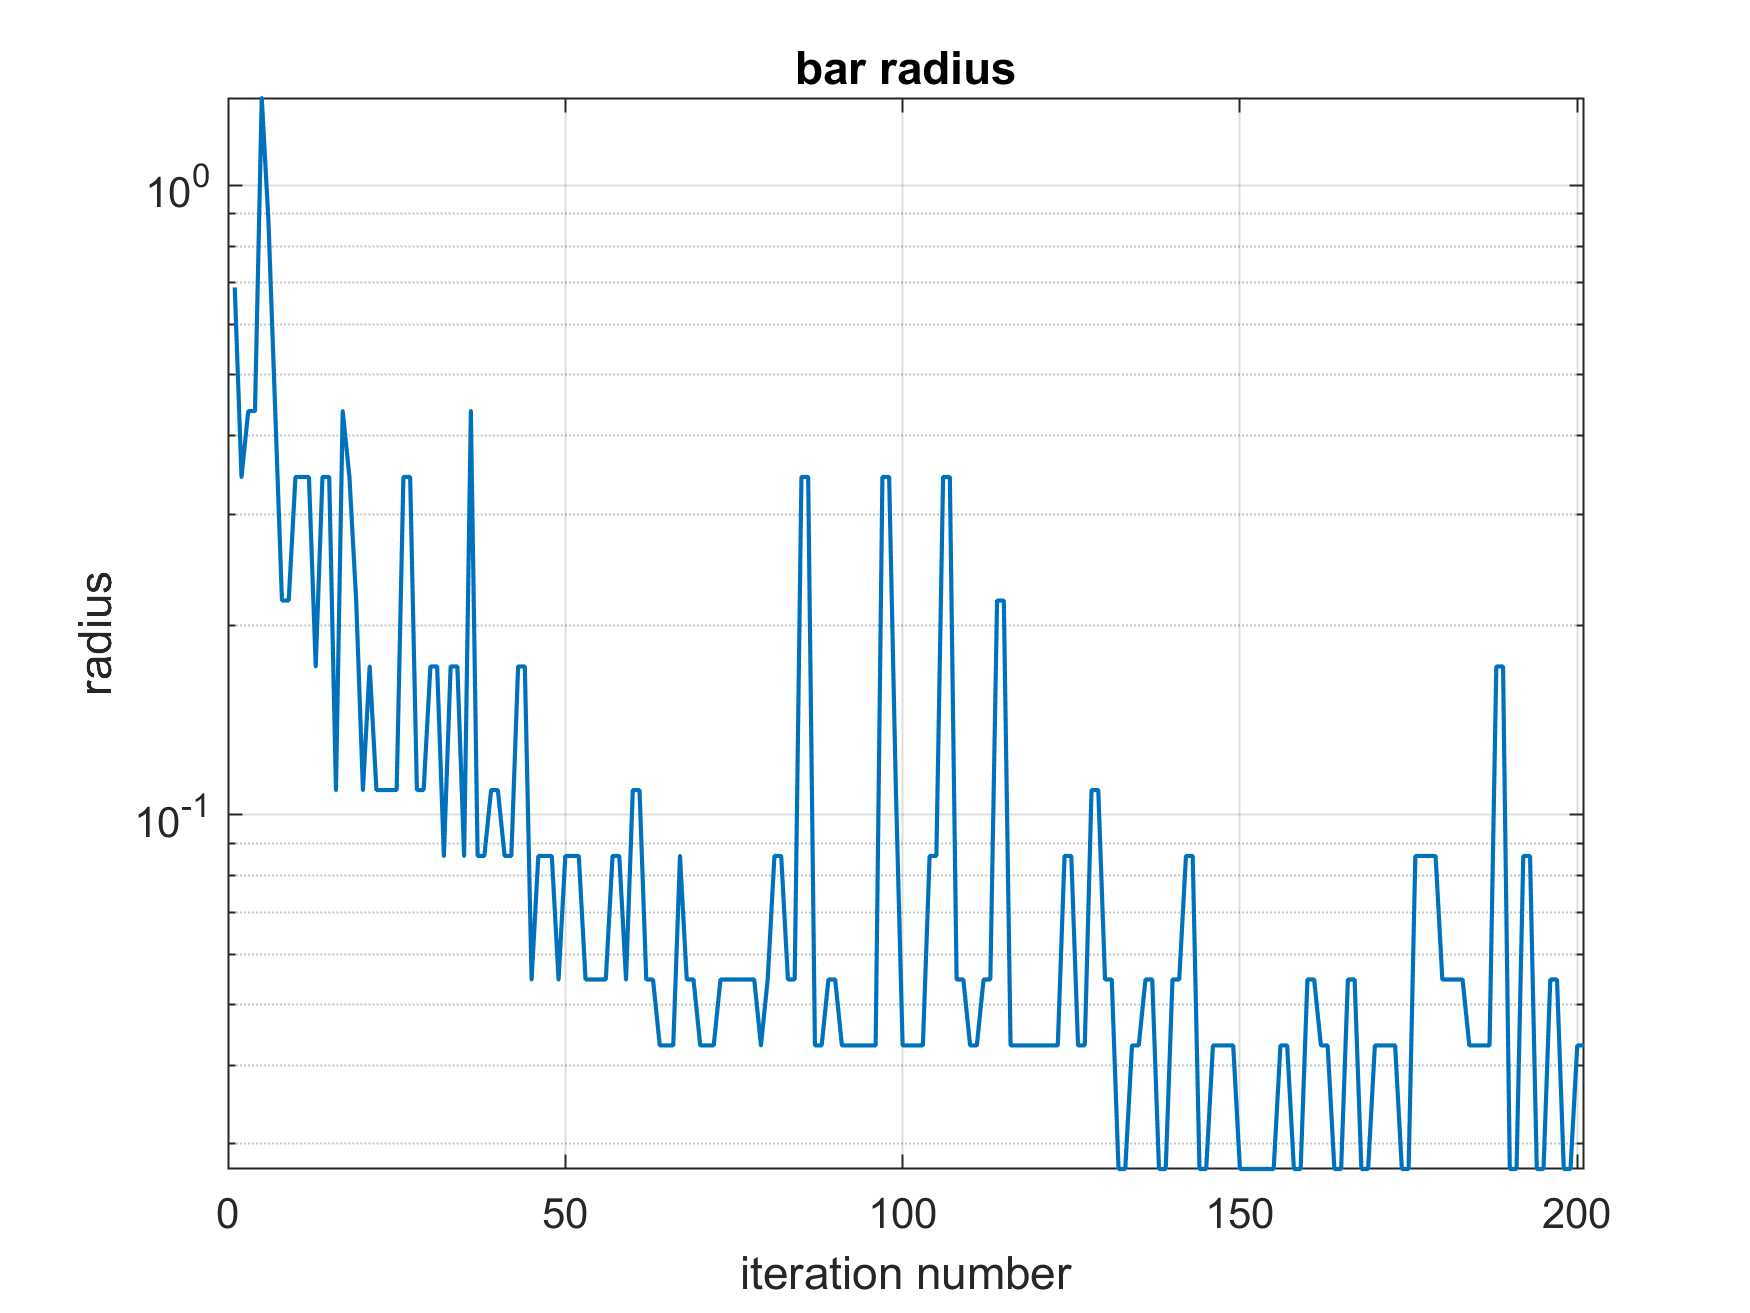
\includegraphics[width=13cm]{img/bar_rad.png}
    \caption{Радиусы рабочих брусов для функции МакКормика (\ref{macCorm})}
    \label{fig:mcRad}
\end{figure}
\subsubsection{Функция с несколькими экстремумами}
Для функции (\ref{Himmel}) в качестве начального приближения был выбран брус $\begin{pmatrix}
[-5,\: 5]\\
[-5,\: 5]
\end{pmatrix}$.
\begin{figure}[H]
    \centering
    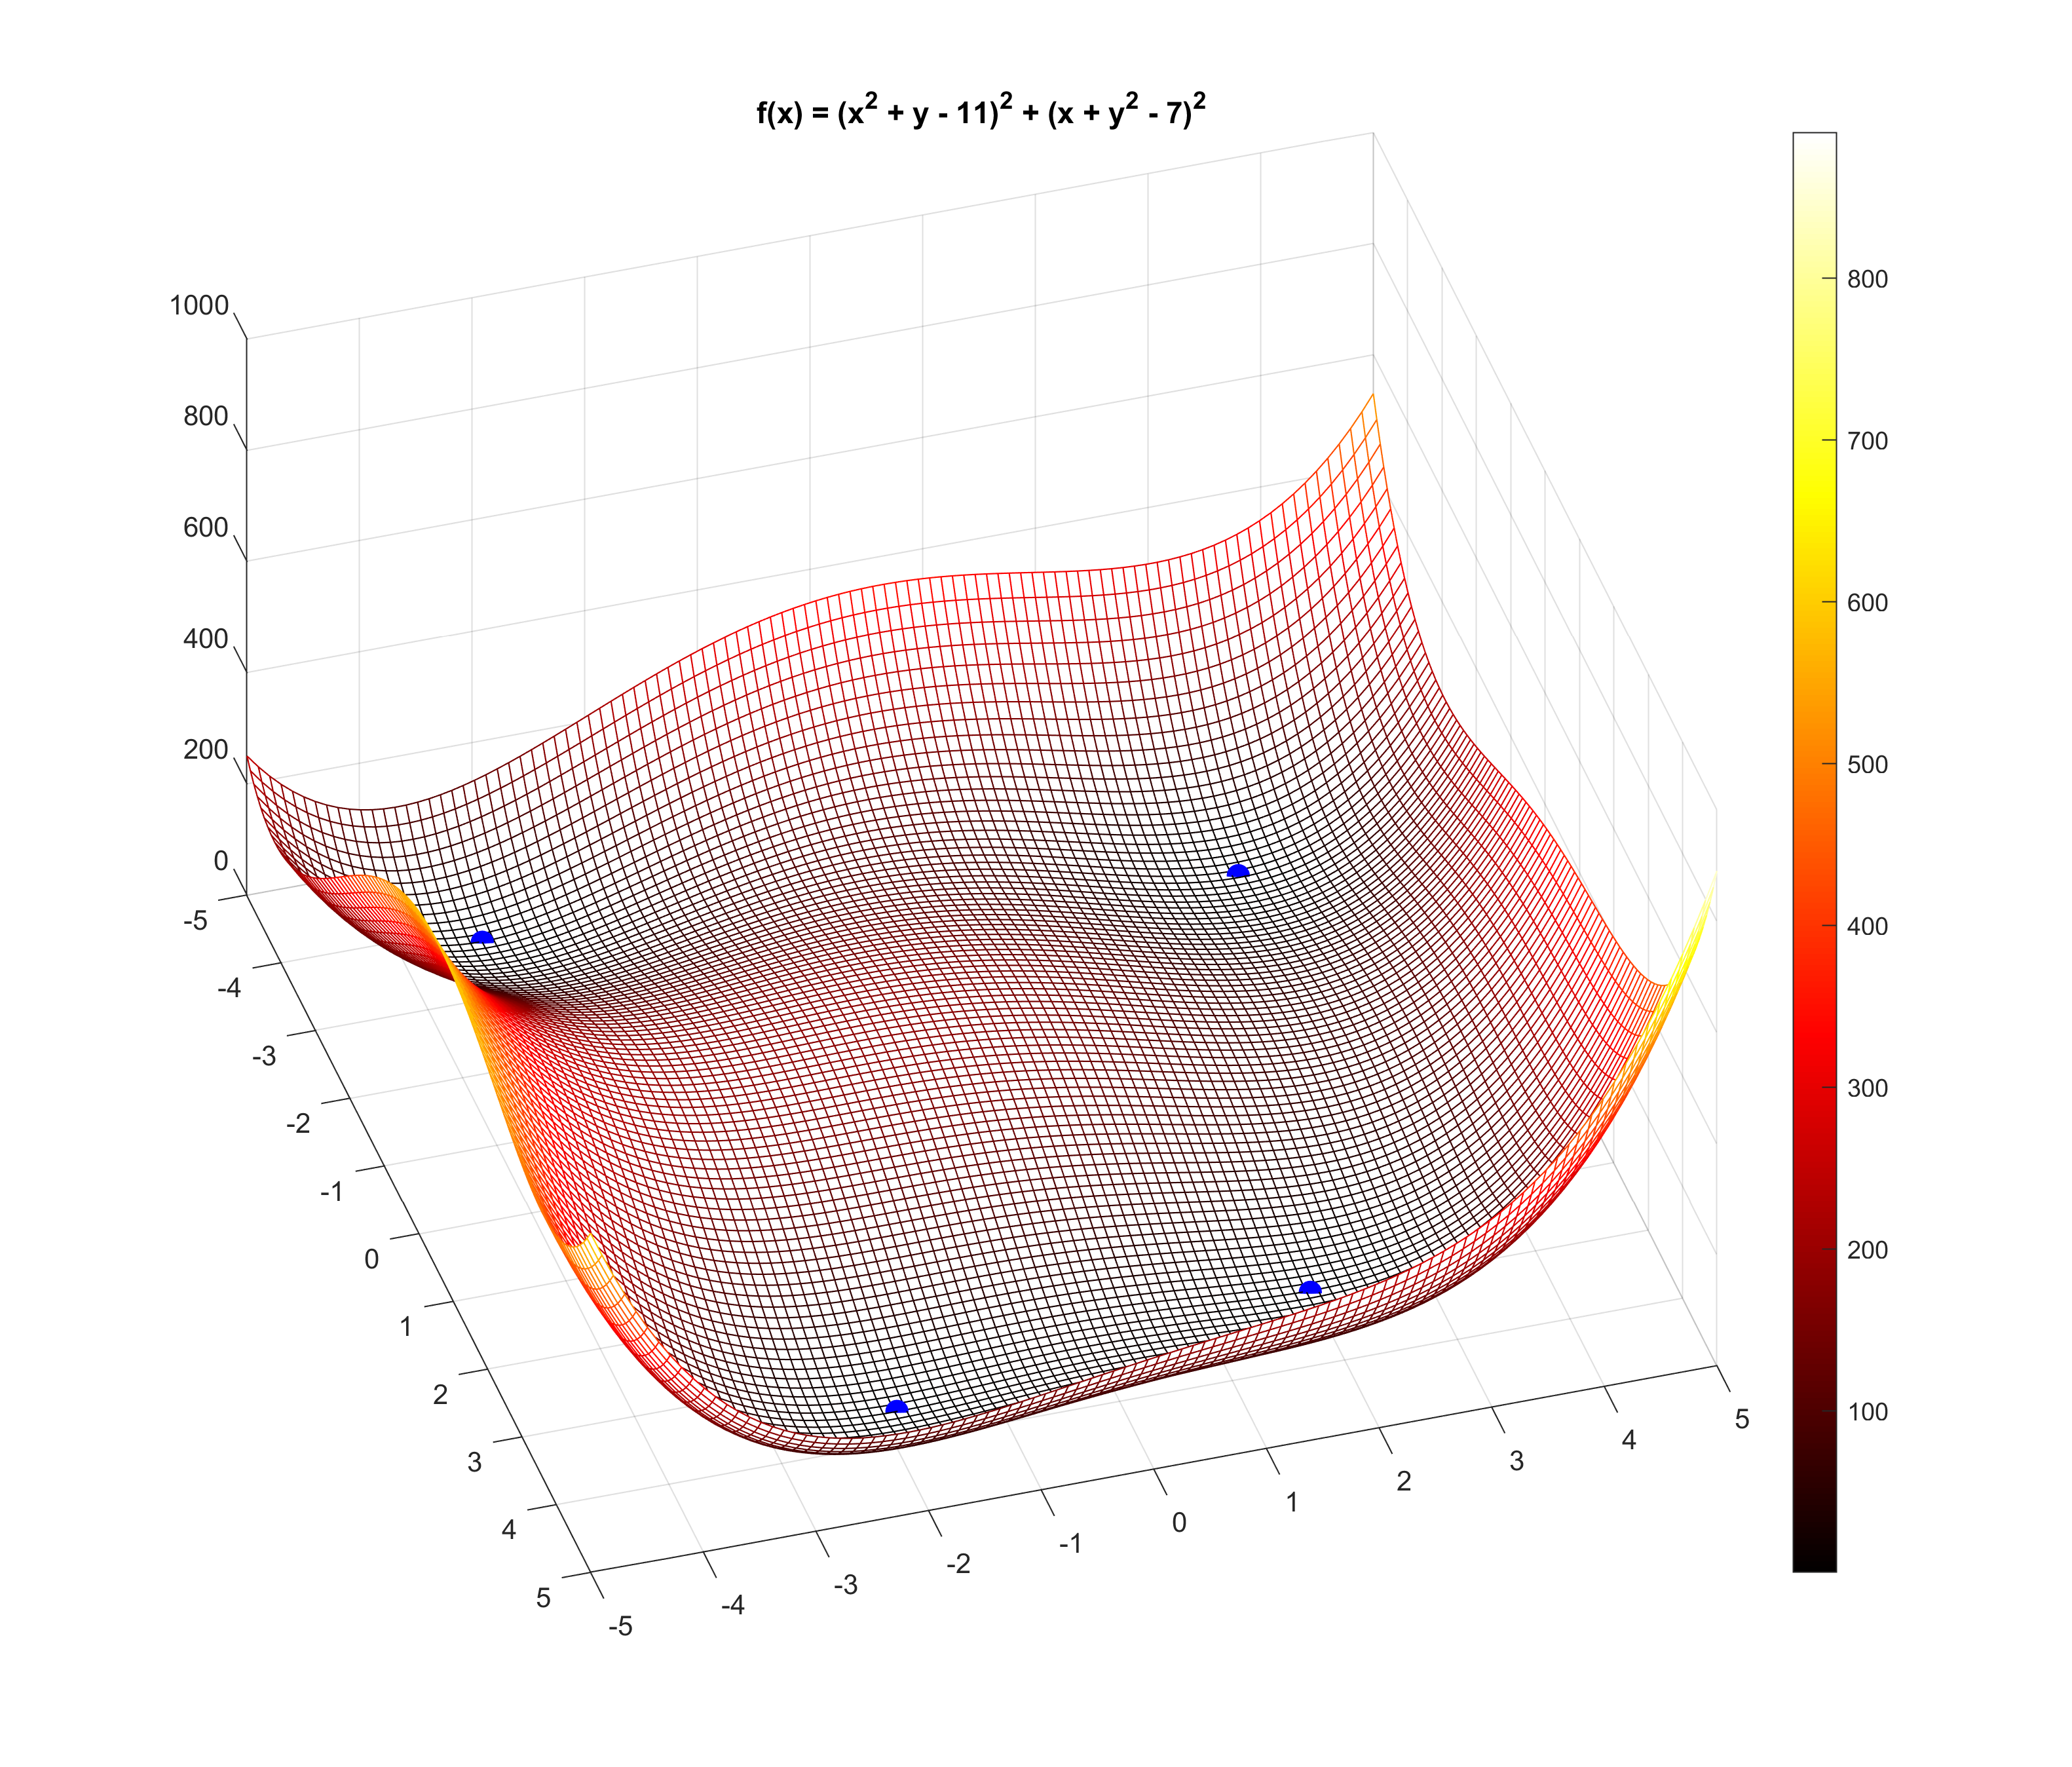
\includegraphics[width=13cm]{img/himmel3d.png}
    \caption{График функции Химмельблау (\ref{Himmel})}
    \label{fig:himmel}
\end{figure}
Функция содержит 4 глобальных экстремума в точках $(3, 2)$, $(-2.8051, 3.1313)$, $(-3.7793, -3.2831)$, $(3.5844, -1.8481)$, отмечены на графике синими точками. Получены следующие результаты:
\begin{figure}[H]
    \centering
    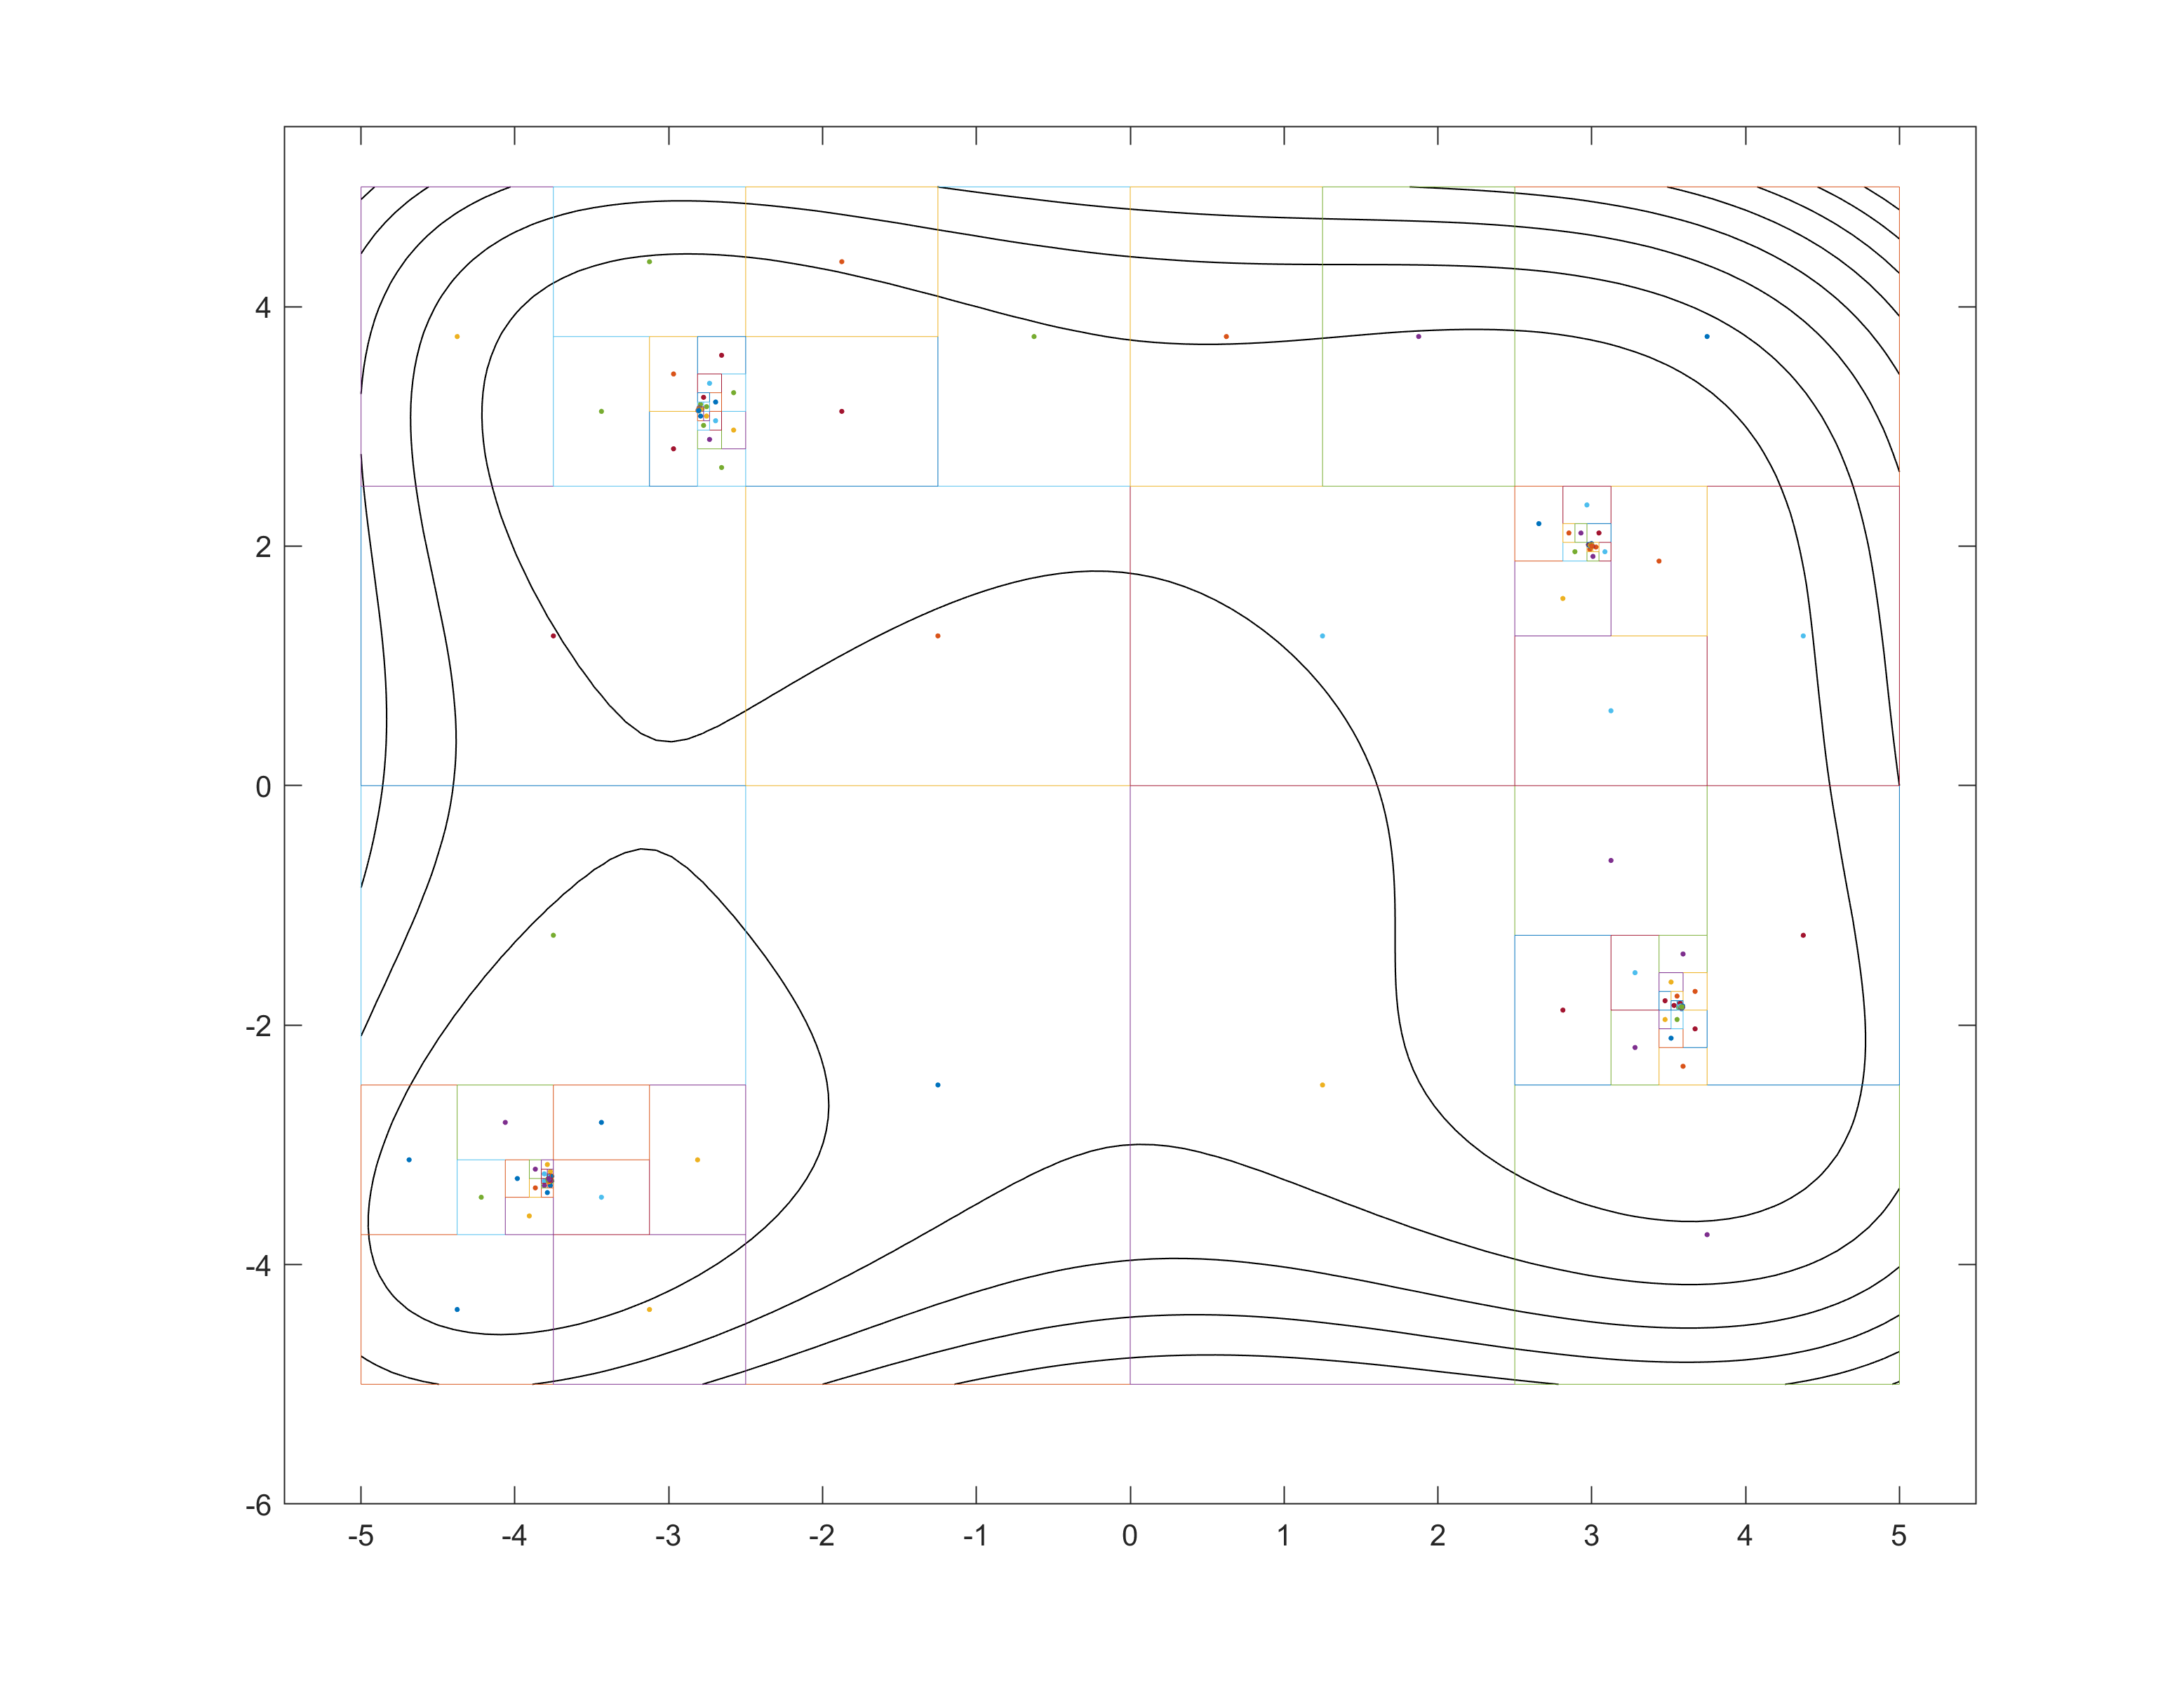
\includegraphics[width=15cm]{img/HimmelOptim.png}
    \caption{Иллюстрация работы алгоритма для функции Химмельблау (\ref{Himmel})}
    \label{fig:himOpt}
\end{figure}
Возле всех 4 минимумов наблюдается сгущение брусьев. В качестве решения получен вырожденный брус $\mathbf{x}\approx\begin{pmatrix}
[   3,\:    3]\\ 
[   2,\:   2]
\end{pmatrix}$, являющийся точным (считая до $10^{-5}$) расположением одного из экстремумов, $f(\mathbf{x})\approx0$. График расстояния до экстремума построен для ближайшего на каждой итерации экстремума.
\begin{figure}[H]
    \centering
    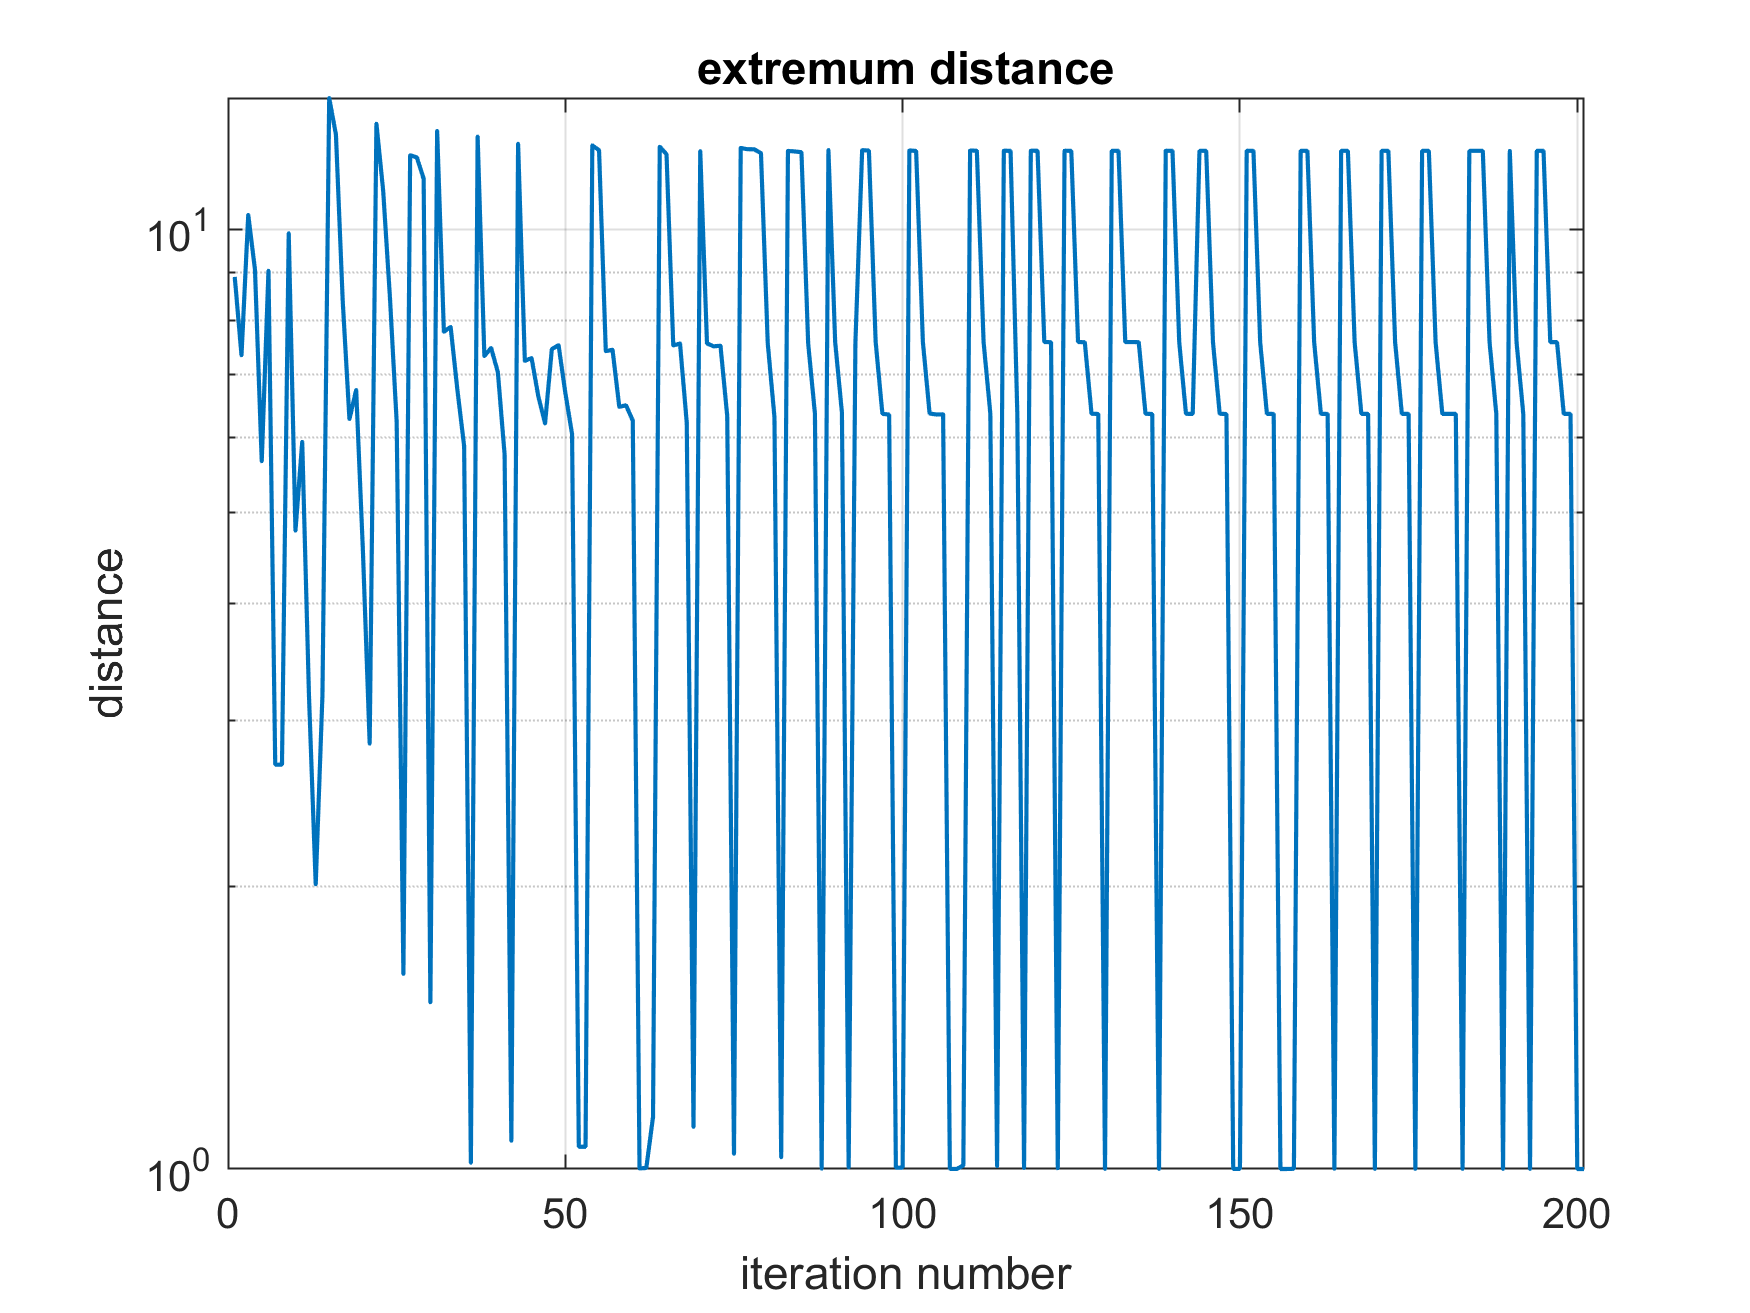
\includegraphics[width=15cm]{img/extr_dist_himmel.png}
    \caption{Расстояние до точки экстремума для функции Химмельблау (\ref{Himmel})}
    \label{fig:himExtr}
\end{figure}
\begin{figure}[H]
    \centering
    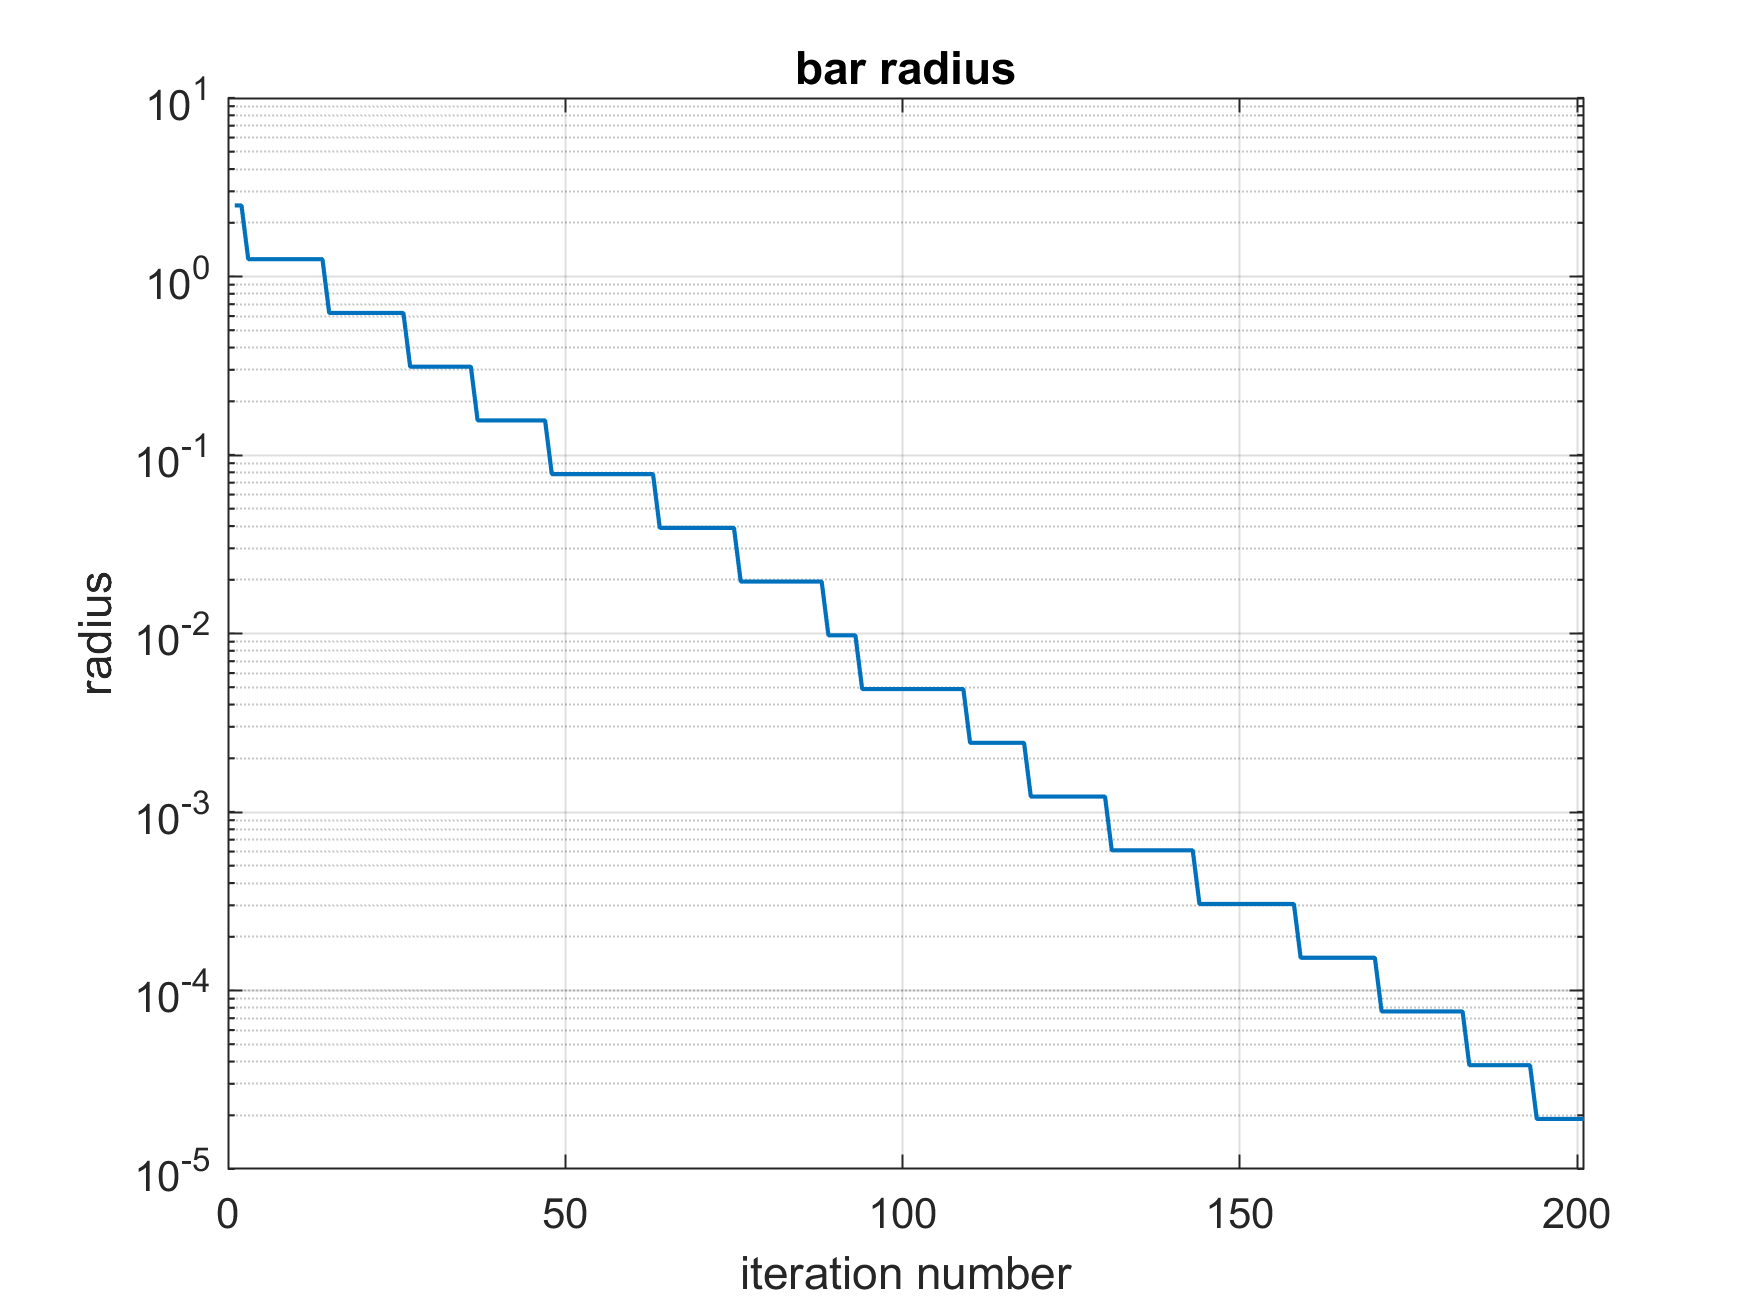
\includegraphics[width=15cm]{img/bar_rad_himmel.png}
    \caption{Радиусы рабочих брусов для функции Химмельблау (\ref{Himmel})}
    \label{fig:radHimmel}
\end{figure}
\section{Обсуждение}
\begin{enumerate}
    \item Переход от задачи (\ref{mat:reg}) к задаче (\ref{math:tom}) сопряжен с введением дополнительных интервальных величин в матрицу, что резко увеличивает сложность определения ее особенности. Более того, из полученных результатов можно сделать вывод, что матрицу $\mathbf{A}$ проще сделать особенной, чем $\mathbf{X}$, так как допуск на значения $\varepsilon$, при которых матрица сохраняет свою неособенность, стал меньше.
    \item При переходе от линейной регрессии к полиномиальной интервалы в столбцах матрицы $\mathbf{X}$ будут умножаться сами на себя, увеличивая таким образом собственный радиус. В данной конкретной задаче уже при достижении степени полинома 2 мы получим особенную матрицу $\forall\varepsilon>0$, так как два первых столбца будут содержать вырожденную точечную матрицу $\left(\begin{smallmatrix}1&1\\1.1&1.1\end{smallmatrix}\right)$. В общем случае довольно сложно что-либо сказать, потому что операция произведения для неположительных интервалов выглядит нетривиально. Тем не менее, опираясь сделанный вывод о переходе от задачи регрессии к задаче томографии, можно сделать предположение, что введение дополнительных интервальных величин в исходную матрицу сузит множество $\varepsilon$, для которых матрица будет неособенной.
    \item В задаче (\ref{math:tom}) результаты, полученные с помощью критерия Баумана, не противоречат результатам, посчитанным с помощью признака Румпа. Более того, в данной задаче по результатам признака Румпа можно дать очень точную оценку значениям $\varepsilon$, при которых матрица $\mathbf{A}$ может стать особенной. Хотя вообще говоря, признак Румпа задает только достаточные условия неособенности, что становится видно после его применения на задаче регрессии.
    \item Для функции МакКормика рассматриваемый алгоритм нахождения минимума функции дал правильную оценку самого значения минимума функции: $-1.9133\in[-2.3019,\:-1.3809]$, но при этом не смог обеспечить сходимости к его точке: $\left(\begin{smallmatrix}
    -0.5471\\ -1.5471
    \end{smallmatrix}\right)\notin \left(\begin{smallmatrix}
    [   -0.3829,\:    -0.2968]\\ 
[   -1.5782,\:   -1.4687]
    \end{smallmatrix}\right)$. Для функции Химмельблау была получено точечная оценка положения одного из экстремумов, причем довольно точная.
    \item Опираясь на графики (\ref{fig:mcExtr}) и (\ref{fig:mcRad}), можно сделать вывод, что на функции (\ref{macCorm}) метод действительно не обеспечивает сходимость к точке экстремума (во всяком случае за конечное число итераций): радиус брусов имеет более высокий порядок малости нежели расстояние до экстремума. Скачкообразное поведение графиков объясняется самим алгоритмом: ведущий брус, который будет далее дробиться, выбирается на каждой итерации путем полного итерирования по рабочему списку, то есть сам автор алгоритма предусматривал, что последний рассмотренный брус может не быть оптимальным, и что необходимо проводить по сути полный перебор рабочего списка в поисках лучшей оценки значения минимума функции. По этой причине монотонного убывания не наблюдается ни на одном из данных графиков.
    \item На функции Химмельблау (\ref{Himmel}) метод показал монотонное убывание радиусов брусов (\ref{fig:radHimmel}) и сошелся к вырожденному брусу, довольно точно описывающему реальное положение точки минимума (примерно до $10^{-5}$). График (\ref{fig:himExtr}) не показывает строгого убывания, что описывается ранее приведенными рассуждениями, однако ведет себя намного лучше, чем аналогичный для фукнции МакКормика (\ref{fig:mcExtr}). По нему видно, что остальные положения экстремумов тоже находятся довольно точно.
    \item Исходя из полученных результатов, можно утверждать, что в общем случае метод пригоден лишь для довольно грубой (причем вряд ли можно провести аналитическую оценку того, насколько грубой) оценки самого значения минимума функции, а не положения точки экстремума, что также подтверждается сигнатурой его функции: на выход выдается лишь нижняя оценка значения минимума и рабочий список брусов, для получения остальных оценок необходимо видоизменять код процедуры или проводить анализ этого списка.
    \item Тем не менее, для функции (\ref{Himmel}) были получены отличные результаты, что дает повод предположить, что плохое поведение метода обусловлено характером функции МакКормика: рассматриваемая область очень пологая и в ней присутствует локальный минимум, в то время, как у функции Химмельблау глобальные минимумы более ярко выражены.
\end{enumerate}
\section*{Исходный код}
С исходным кодом программы и отчета можно ознакомиться в репозитории \url{https://github.com/Stasychbr/IntervalArith}.
\end{document}
